\section{Computation graph creation} \label{sec:cg}
This section formally defines how to build a computation graph from an execution trace of a task parallel program. The formalism is driven by a desire to be general enough to cover any language feature in a task parallel language while being specific enough to precisely define the graph construction. 
The programming model is derived from Bouajjani and Emmi for isolated parallel tasks \cite{bouajjani}. The derivative in this paper allows sharing since programmers use it (intentionally or otherwise). The definition is thus expanded from the original in two ways: first, parallel regions now include a single shared variable that can be accessed by any task with a handle to the region; and second, tasks include additional sets indicating which regions are for reading and which regions are for writing relative to the shared region variable in each region.

The surface syntax for the language is given in \figref{fig:syntax}. A program \textbf{P} is a sequence of procedures. The procedure name $p$ is taken from a finite set of names \texttt{Proc}. Each procedure has a single $L$-type parameter \texttt{l} taken from a finite set of parameter names \texttt{Vars}. The body of the procedure is inductively defined by $s$. The semantics is abstracted over concrete values and operations, so the possible types of \texttt{l} are not specified nor is the particular expression language, $e$, but assume it includes variables references and Boolean values (\textbf{true} and \textbf{false}). The details of either $L$ or $e$ are never relevant for computation graph construction and are thus omitted. The set of all expressions is given by \texttt{Exprs}. Values are given by the finite set \texttt{Vals} and include at least Boolean values. \texttt{Exprs} contain \texttt{Vals} and the \emph{choice operator} $\star$. 

\begin{figure}
  \begin{center}
\[
  \begin{array}{rcl}
\textbf{P} &::=& (\textbf{proc}~p~(\textbf{var}\ \texttt{l} : L)~s)* \\
\textbf{s} &::=& s;~s \alt \texttt{l} := e \alt \texttt{l}(r)\ := e \\
&\alt& \textbf{skip} \alt  \textbf{assume}~e \\
&\alt& \textbf{if}~e~\textbf{then}~s~\textbf{else}~s \alt \textbf{while}~e~\textbf{do}~s \\
&\alt& \textbf{call}~\texttt{l}\ := p~e~\vec{r_\delta}~\vec{r_\omega} \alt \textbf{return}~e \\
&\alt& \textbf{post}~r \leftarrow p~e~\vec{r}~\vec{r_\delta}~\vec{r_\omega}~d \\
&\alt& \textbf{await}~r \alt \textbf{ewait}~r \\
  \end{array}
\]
  \end{center}
  \caption{The surface syntax for task parallel programs.}
  %\vspace{-2em}
  \label{fig:syntax}
\end{figure}

The statements ($s$) of the language denote the behavior of the procedure. Most statements, like the \textbf{if}-statement, \textbf{;}-statement, and \textbf{while}-statement have their typical meaning. Other statements require further explanations.

Statements are divided into the concurrent statements (\textbf{post}-statement, \textbf{await}-statement and \textbf{ewait}-statement) and sequential statements (everything else).  Let \texttt{Regs} be a finite set of region identifiers. Associated with each region $r$ is a single variable referenced in the surface syntax by $\texttt{l}(r)$. A task is posted into a region $r$ by indicating the procedure $p$ for the task with an expression for the local variable value $e$, three lists of regions from $\texttt{Regs}^\ast$ (i.e., the Kleene closure on \texttt{Regs}), and a return value handler $d$. For the region lists, $\vec{r}$ are regions whose ownership is transferred from the parent to the new child task (i.e., the child now owns the tasks in those regions), $\vec{r_\delta}$ are regions in which the new task can read the region variables, and $\vec{r_\omega}$ are regions in which the task can write region variables. Let \texttt{Stmts} be the set of all statements and let $\texttt{Rets} \subseteq (\texttt{Vals} \rightarrow \texttt{Stmts})$ be the set of return value handlers. The handler $d$ associates the return value of the procedure with a user defined statement. 

The \textbf{await} and \textbf{ewait} statements synchronize a task with the sub-ordinate tasks in the indicated region. Intuitively, when a task calls \textbf{await} on region $r$, it is blocked until all the tasks it owns in $r$ finish execution. Similarly, when a task issues an \textbf{ewait} with region $r$, it is blocked until one task it owns in $r$ completes. The rest of the tasks in the region  $r$ continue their execution normally and are joined when another \textbf{ewait} or \textbf{await} statement is issued by the parent task. A task is termed \emph{completed} when its statement is a \textbf{return}-statement. 

The \textbf{assume}-statement blocks a task until its expression $e$ evaluates to \textbf{true}. By way of definition, \textbf{call}, \textbf{return}, \textbf{post}, \textbf{ewait} and \textbf{await} are \emph{inter-procedural} statements. All other statements are \emph{intra-procedural}.

\begin{figure}
%\vspace{-1em}
  \begin{center}
    \begin{lstlisting}[mathescape=true]
  proc main (var n : int)
  	n := 1;
	post $r_1 \leftarrow p_1~n~\varepsilon~(r_1)~(r_1)~\lambda v.n := n + v$;
	post $r_1 \leftarrow p_2~n~\varepsilon~(r_1)~(r_1)~\lambda v.n := n + v$;
	await $r_1$
  proc $p_1$ (var n : int)
  	$\texttt{l}(r_1) := \texttt{l}(r_1) + n$;
	return (n + 1)
  proc $p_2$ (var n : int)
  	$\texttt{l}(r_1) := \texttt{l}(r_1) + n$;
	return (n + 2)
\end{lstlisting}
  \end{center}
%  \vspace{-2em}
  \caption{A simple example of a task parallel program.}
  \label{fig:hj-async-finish}
%  \vspace{-1em}
\end{figure}

\figref{fig:hj-async-finish} shows a simple example program. The main task posts two new tasks $t_1$ and $t_2$ executing procedures $p_1$ and $p_2$ in region $r_1$. $\varepsilon$ denotes an empty region sequence. The tasks $t_1$ and $t_2$ have access to the variable $r_1$. The $main$ task awaits the completion of $t_1$ and $t_2$. The return value handler of procedure $main$ takes the value returned by the tasks $t_1$ and $t_2$ and updates the value of $n$. The computation graph for this program is that in \figref{fig:cg}.

%\subsection{Tree-based Semantics}

The semantics is defined over trees of procedure frames to represent the parallelism in the language rather than stacks which are inherently sequential. That means that the frame of each posted task becomes a child to the parent's frame. The parent-child relationship is transferred appropriately with task passing or when a parent completes without synchronizing with its children. The evolution of the program proceeds by a task either taking an intra-procedural step, posting a new child frame, or removing a frame for a synchronized completed task.

A task $t = \tuple{\ell, s, d, \vec{r_\delta}, \vec{r_\omega}, n}$ is a tuple containing the valuation of the procedure local variable \texttt{l}, along with a statement $s$, a return value handler $d$, a list of regions that it may use for read variables, a list of regions it may use for write variables, and an associated node in the computation graph for this task. When a procedure $p$ is posted as a task, the statement $s$ is the statement defined for the procedure $p$---recall that statements are inductively defined. 

A \emph{tree configuration}, $c = \tuple{t,m}$, is an inductively defined tree with task-labeled vertexes, $t$, and region labeled edges given by the \emph{region valuation} function, $m : \texttt{Regs} \rightarrow \mathbb{M}[\texttt{Configs}]$, where \texttt{Configs} is the set of tree configurations and $\mathbb{M}[\texttt{Configs}]$ are configuration multi-sets. For a given vertex $c = \tuple{t,m}$, $m(r)$ returns the collection of sub-trees connected to the $t$-labeled root by $r$-labeled edges.

The semantics relies on manipulating region valuations for task passing between parents and children. For two region valuations $m_1$ and $m_2$, the notation $m_1 \cup m_2$ is the multi-set union of each valuation. Further, the notation $m\ |_{\vec{r}}$ is the projection of $m$ to the sequence $\vec{r}$ defined as $m\ |_{\vec{r}}(r^\prime) = m(r^\prime)$  when $r^\prime$ is found somewhere in $\vec{r}$, and $m\ |_{\vec{r}}(r^\prime) = \emptyset$ otherwise. 

Let $\llbracket \cdot \rrbracket_e$ be an evaluation function for expressions without any program or region variables such that $\llbracket \star \rrbracket_e = \texttt{Vals}$, and let $\ell(r)$ denote the value of the region variable in $r$. For convenience in the semantics definition, an evaluation function is defined over a task $t$ that enforces the read rights assigned to the task:
\begin{eqnarray*}
  e(t) &=& e(\tuple{\ell, s, d, \vec{r_\delta}, \vec{r_\omega}, n}) \\
  &=& e(\ell, \vec{r_\delta}) \\
  &=& e(\ell, r_0, r_1, \ldots) \\
  &=& \llbracket e[\ell / \texttt{l},\ell(r_0) / \texttt{l}(r_0), \ell(r_1) / \texttt{l}(r_1), \ldots]  \rrbracket_e
  \end{eqnarray*}
If $e[\ell / \texttt{l},\ell(r_0) / \texttt{l}(r_0), \ell(r_1) / \texttt{l}(r_1), \ldots]$ has any free variables, then by definition, \\
$\llbracket e[\ell / \texttt{l},\ell(r_0) / \texttt{l}(r_0), \ell(r_1) / \texttt{l}(r_1), \ldots]  \rrbracket_e$ has no meaning and is undefined (i.e., $e(t) = \emptyset$). e(t) is set-valued, although most expressions evaluate to singletons. As a final convenience for dealing with expressions in the semantics when constructing computation graphs, let the set of regions whose variables appear in $e$ be denoted by $\eta(e)$. 

Contexts are used to further simplify the notation needed to define the semantics.  A \emph{configuration context}, $C$, is a tree with task-labeled vertexes, region-labeled edges and a single $\diamond$-labeled leaf. The notation $C[c]$ denotes the configuration obtained by substituting a configuration $c$ for the unique $\diamond$-labeled leaf of $C$. The configuration isolates individual task transitions (e.g., $C[\tuple{t,m}] \rightarrow C[\tuple{t^\prime,m}]$ denotes an intra-procedural transition on a task). Similarly, a \emph{statement context} is given as $S = \diamond ; s_1; \dots ;s_i$ and $S[s]$ indicates that $\diamond$ is replaced by $s$ where $s$ is the next statement to be executed. A \emph{task statement context}, $T = \tuple{\ell,  S, d, \vec{r_\delta}, \vec{r_\omega}, n}$ is a task with a statement context in place of a statement, and likewise $T[s]$ indicates that $s$ is the next statement to be executed in the task. Like configuration contexts, task statement contexts isolate the statement to be executed (e.g., $C[\tuple{T[s_1],m}] \rightarrow C[\tuple{T[s_2],m}]$ denotes an intra-procedural transition that modifies the statement in some way). For convenience, $e(t)$ is naturally extended to use contexts as indicated by $e(T)$. 

As indicated previously, a task $t$ is completed when its next to be executed statement $s$ is \textbf{return} $e$. The set of possible return-value handler statements for $t$ is $\mathrm{rvh}(t) = \{d(\ell) \mid \ell \in e(T)\}$ given the task's context. By defnition, $\mathrm{rvh}(t) = \emptyset$ when $t$ is not completed or $e(T)$ is undefined. 

The initial condition for a program $\iota = \tuple{p, \ell}$ is an initial procedure $p \in \texttt{Procs}$ and an initial value $\ell \in \texttt{Vals}$. The initial configuration is created from $\iota$ as $c = \tuple{\tuple{\ell, s_p, d, \vec{r_\delta}, \vec{r_\omega}, n}, m}$, where $s_p$ is the statement for the procedure $p$, $d$ is the identity function (i.e., $\lambda v.v$), $\vec{r_\delta}$ list regions whose variables are read by $p$, $\vec{r_\omega}$ lists regions whose variables are written by $p$, $n$ is a fresh node for the computation graph (i.e., $n = \mathrm{fresh}()$), and $\forall r \in \texttt{Regs}, m(r) = \emptyset$.

The semantics is now given as a set of transition rules relating tree configurations. The rules assume the presence of a global computation graph, $G = \tuple{N, E, \delta, \omega}$, that is updated as part of the transition. The initial graph contains a single node $N = \{n\}$ from the initial configuration, no edges ($E = \emptyset$), and no read/write information ($\delta(n) = \emptyset$ and $\omega(n) = \emptyset$).

\begin{figure}
  \begin{center}
    \mprset{flushleft}
    \begin{mathpar}
      \inferrule[Call]
                {
                }
                {
                  C[T[\textbf{call}~\texttt{l}\ := p~e~\vec{r_\delta}~\vec{r_\omega}], m] \rightarrow \\
                  C[T[\textbf{post}~r_\mathit{call}\leftarrow p~e~\varepsilon~\vec{r_\delta}~\vec{r_\omega}~\lambda v.\texttt{l} := v;~ \textbf{ewait}~r_\mathit{call}], m]
               }
      \and
      \inferrule[Post]
                {
                  n_0^\prime = \mathrm{fresh}() \\
                  n_1 = \mathrm{fresh}() \\
                  N = N \cup \{n_0^\prime, n_1\} \\
                  E = E \cup \{\tuple{n_0, n_0^\prime}, \tuple{n_0, n_1}\}\\\\
                  \ell \in e(\ell^\prime,\vec{r_\delta}^\prime) \\
                  \delta = \delta \cup (n_0 \mapsto \eta(e))\\\\
                  m^\prime = (m \setminus m |_{\vec{r}}) \cup
                  (r \mapsto \tuple{
                    \tuple{\ell, s_p, d, \vec{r_\delta}, \vec{r_\omega},n_1},m|_{\vec{r}}})
                }
                {
                  C[\tuple{\ell^\prime,
                      S[\textbf{post}~r \leftarrow p~e~\vec{r}~\vec{r_\delta}~\vec{r_\omega}~d],\vec{r_\delta}^\prime,\vec{r_\omega}^\prime,d^\prime, n_0}, m] \rightarrow \\
                  C[\tuple{\ell^\prime,
S[\textbf{skip}],\vec{r_\delta}^\prime,\vec{r_\omega}^\prime,d^\prime, n_0^\prime}, m^\prime]
                }
      \and
      \inferrule[Ewait]
                {
                  n^\prime = \mathrm{fresh}() \\
                  N = N \cup \{n^\prime\} \\
                  E = E \cup \{\tuple{n, n^\prime}, \tuple{n(t_2),n^\prime}\} \\\\
                  m_1 = (r \mapsto \tuple{t_2,m_2}) \cup m_1^\prime \\
                  s \in \mathrm{rvh}(t_2) 
                }
                {
                  C[\tuple{\ell,
S[\textbf{ewait}~r],\vec{r_\delta},\vec{r_\omega},d, n}, m_1] \rightarrow \\
                  C[\tuple{\ell,
S[s],\vec{r_\delta},\vec{r_\omega},d, n^\prime}, m_1' \cup m_2]
          }
      \and
      \inferrule[Await-next]
                {
                  n^\prime = \mathrm{fresh}() \\
                  N = N \cup \{n^\prime\} \\
                  E = E \cup \{\tuple{n, n^\prime}, \tuple{n(t_2),n^\prime}\} \\
                  m_1 = (r \mapsto \tuple{t_2,m_2}) \cup m_1^\prime \\
                  s \in \mathrm{rvh}(t_2) 
                }
                {
                  C[\tuple{\ell,
S[\textbf{await}~r],\vec{r_\delta},\vec{r_\omega}, d, n}, m_1] \rightarrow \\
                  C[\tuple{\ell,
S[s;~\textbf{await}~r],\vec{r_\delta},\vec{r_\omega},d, n^\prime}, m_1' \cup m_2]
                }
      \and
      \inferrule[Await-done]
                {
                  m(r) = \emptyset
                }
                {
                  C[T_1[\textbf{await}~r] , m] \rightarrow
                  C[T_1[\textbf{skip}], m]
                }
\end{mathpar}
  \end{center}
  \caption{The transition rules for the inter-procedural statements.}
%    \vspace{-2em}
  \label{fig:inter}
    \label{fig:semantics}
\end{figure}

\begin{figure}
  \begin{center}
     \subfigure[Task creation.]{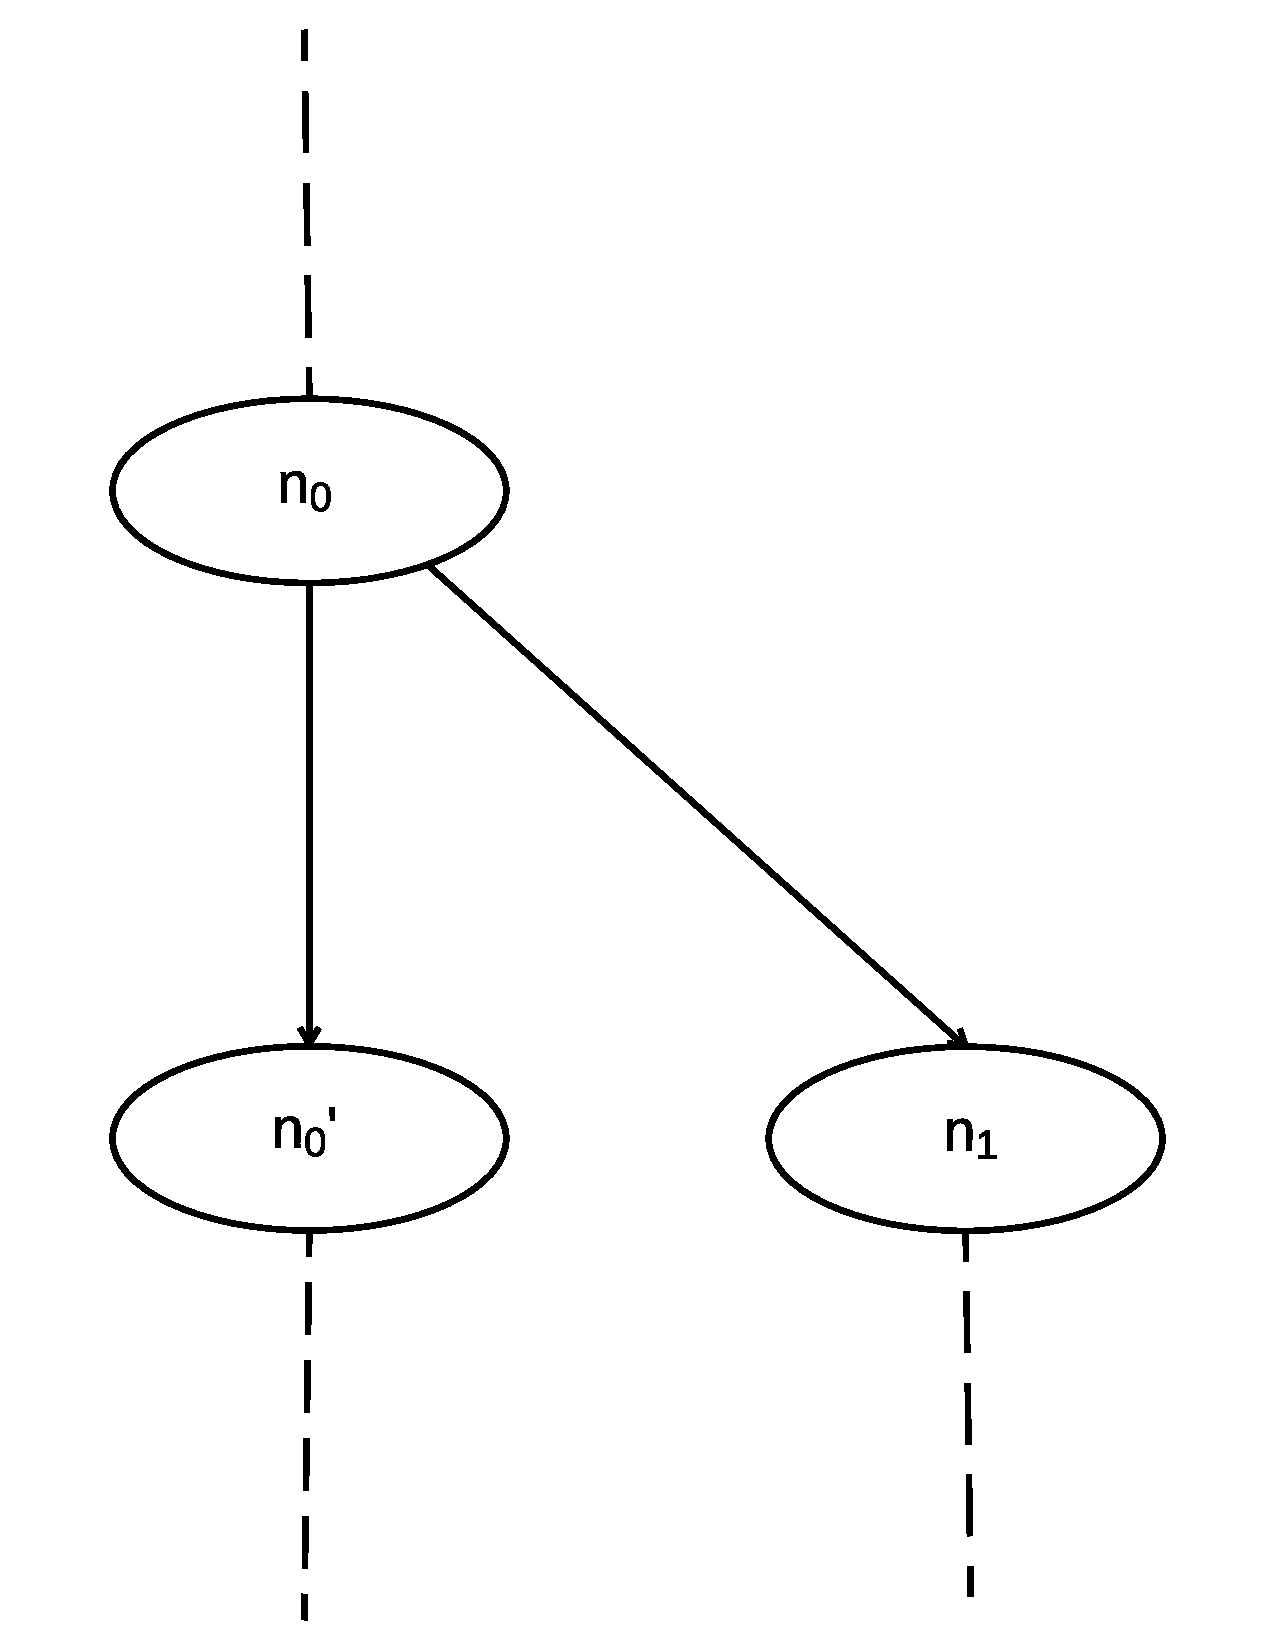
\includegraphics[scale=0.15]{../figs/Fig1-a.pdf}}
     \subfigure[Task synchronization.]{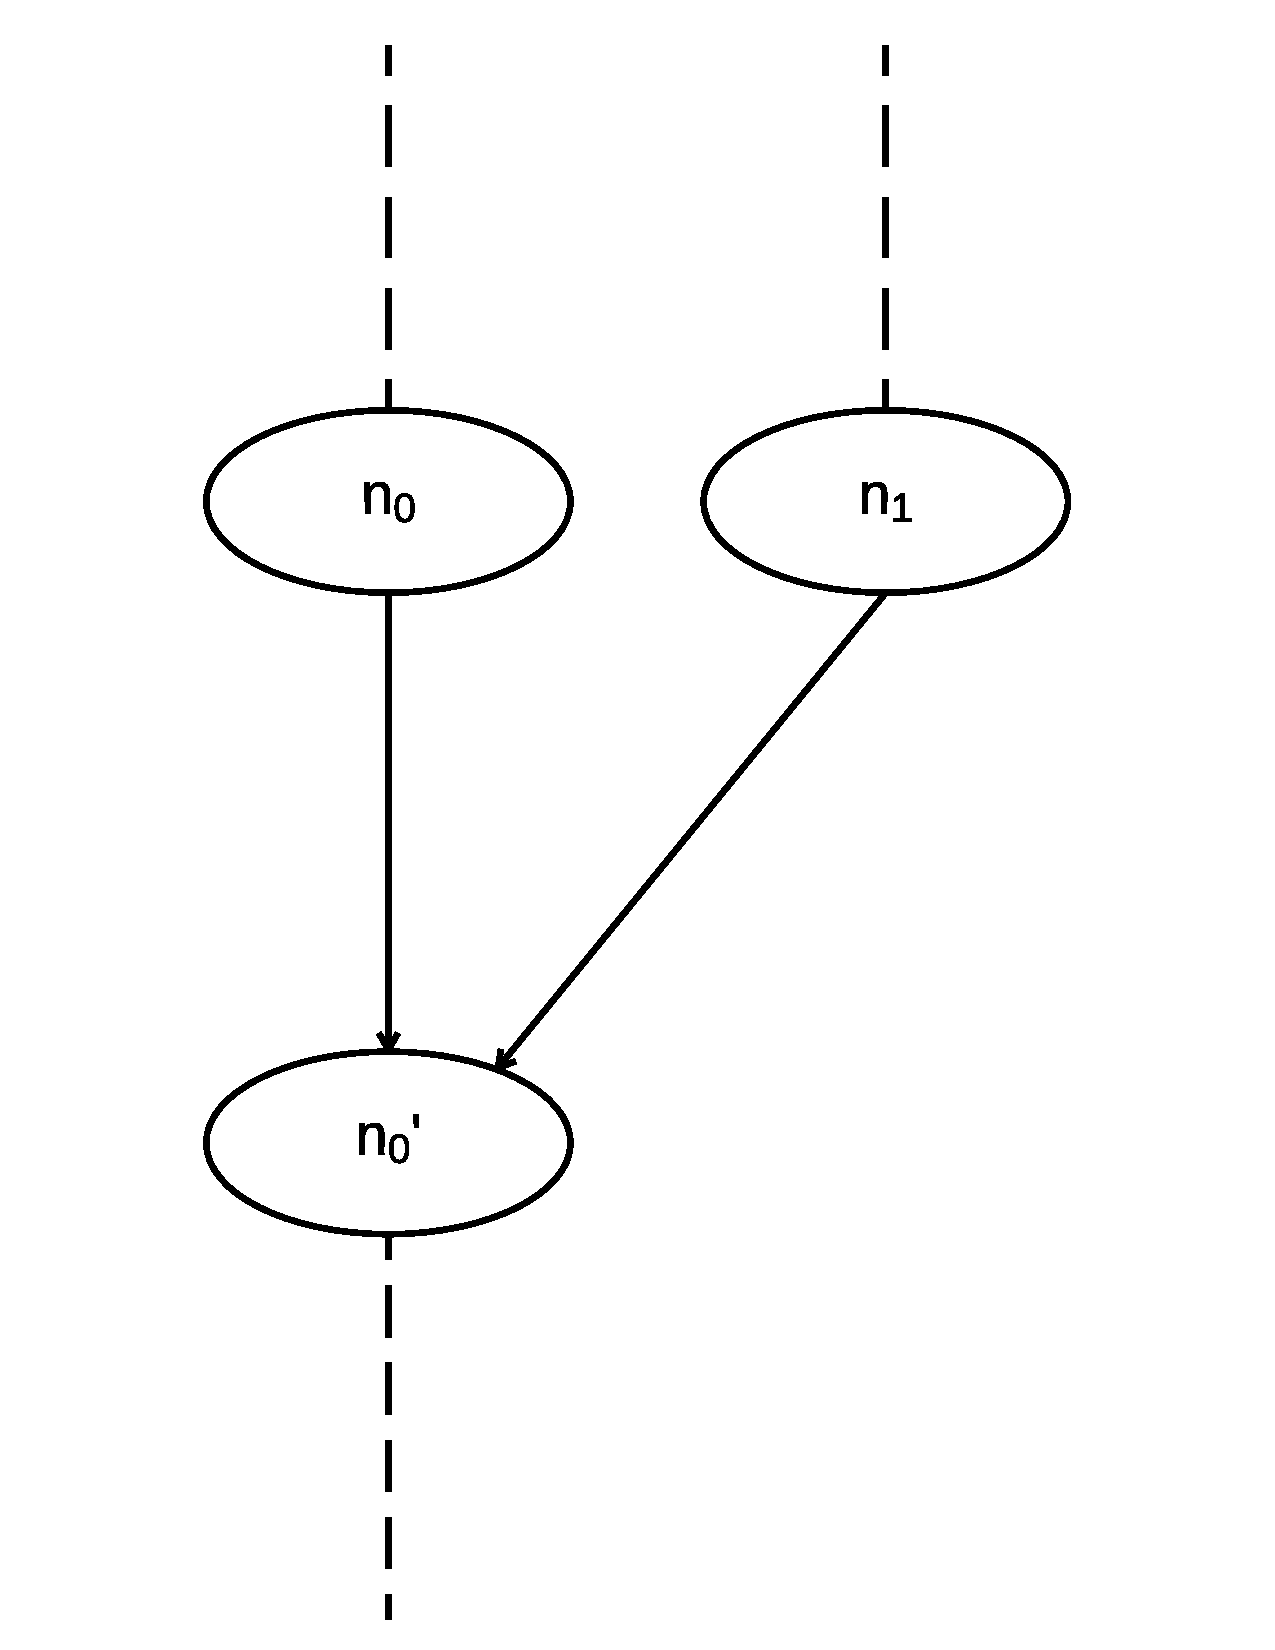
\includegraphics[scale=0.15]{../figs/Fig1-b.pdf}}
  \caption{Steps involved in computation graph creation.}
%  \vspace{-2em}
   \label{fig:cgcreation}
   \end{center}
\end{figure}

The intra-procedural transition rules are omitted for space but are defined in the usual way. \figref{fig:inter} shows semantics for the inter-procedural statements. The notation, $\delta = \delta \cup (n \mapsto \eta(e))$, is understood to update $\delta$ such that $n$ additionally maps to $\eta(e)$. A function notation is adopted to access the tuple $T = \tuple{\ell,  S, d, \vec{r_\delta}, \vec{r_\omega}, n}$. For example, $\vec{r_\omega}(T)$ indicates the read-region vector in the task or task context.

The \textbf{call} statement is interpreted as a \textbf{post} followed by \textbf{ewait} on some region $r_{call}$. This region $r_{call}$ is exclusive to the task calling the procedure and cannot be used to post new tasks into this region. A call statement does not allow ownership of any tasks to be passed to the newly created task. The region variables that are available to this task for reading and writing are denoted by $\vec{r_\delta}$ and $\vec{r_\omega}$ respectively.

The \textsc{Post} rule is fired when the task forks to create a new child task that potentially runs in parallel with the parent task. When a task $t_1$ executes a \textbf{post} statement, two fresh nodes $n_0^\prime$ and $n_1$ are added to the graph. Node $n_0^\prime$ represents the statements following \textbf{post} and $n_1$ represents the statements executed by $t_2$. The current node $n_0$ of $t_1$ is connected to $n_0^\prime$ and $n_1$ as shown in \figref{fig:cgcreation}(a). The read set $\delta$ of node $n_0$ is updated to additionally map to the regions in $\eta(e)$ (i.e., the regions referenced in the expression $e$). The current node of $t_1$ changes to $n_0^\prime$ after the transition. The region mapping $m$ of task $t_1$ is updated by removing the configurations of regions whose ownership is passed to the newly created task $t_2$ and adding a new configuration that consists of the task $t_2$ along with the regions it now owns.

The \textsc{Ewait} rule blocks the execution of the currently executing task until a task in the indicated region completes. The choice of completed task, $t_2$, in the region is non-deterministic. A node $n^\prime$ is added to the graph to act as a join node. It captures the subsequent statements of $t_1$ after the \textbf{ewait} statement finishes. The current node $n$ of task $t_1$ and the current node of task $t_2$, denoted by $n(t_2)$ are connected to $n^\prime$ as shown in \figref{fig:cgcreation}(b). The configuration ($r \mapsto \tuple{t_2,m_2}$) is removed from the region valuation $m$ of $t_1$. After the transition, the current node of task $t_1$ is changed to $n^\prime$.  The task $t_1$ is resumed with a return value handler for the completed task ($\mathrm{rvh}(t_2)$) before continuing with its next statement.

The \textsc{Await-Next} rule blocks the execution of the currently executing task $t_1$ until 
%all the tasks whose handles are stored in region $r$ that the task $t_1$ owns are executed to completion. 
all the tasks owned by $t_1$ whose handles are stored in region $r$ complete execution.
The rule is implemented recursively by removing one task from the region at a time and then inserting another \textbf{await}-statement on the same region. A join node $n^\prime$ is added to the graph, the current nodes of $t_1$ and $t_2$ are connected to $n^\prime$ as shown in \figref{fig:cgcreation}(b) and the current node of $t_1$ is changed to $n^\prime$. When task $t_2$ returns a value to $t_1$, $t_1$ executes the statement from the return value handler $\mathrm{rvh}(t_2)$. The \textsc{Await-Done} rule terminates recursion when the region is empty. 

The computation graph for the example in \figref{fig:hj-async-finish} is presented in \figref{fig:cg}. The order of synchronization of tasks $t_1$ and $t_2$ affects the value of the variable $r_1$ in the $main$ task. The return value handlers of the tasks get executed in different orders under different program schedules. This makes the output of the program non-deterministic. In a schedule where task $t_1$ joins $main$ task before $t_2$, the value of $n$ at the end of program execution is 3 and in a schedule where task $t_2$ joins $main$ task before $t_1$, the value of $r_1$ is 2.

\begin{theorem}
Using the tree semantics with Algorithm \ref{algo:drd} to detect data-race in the resulting computation graph is complete for a task parallel program with a given input.
\end{theorem}
\begin{comment}
\begin{proof}

%Proof is available in the longer version of this paper.


The semantics described in \figref{fig:semantics} show how a computation graph is built for a task parallel program from an observed program execution. The nodes in the graph depict the correct partial order between the tasks in the program. Theorem \ref{thm:graph} shows that Algorithm \ref{algo:drd} is sound and complete for a given computation graph. A task parallel program can have different computation graphs based on the schedule followed by the tasks during the program execution. If Algorithm \ref{algo:drd} does not report a race for a computation graph obtained from some execution of the program, data races may still be observed under some other program schedule. Therefore, Algorithm \ref{algo:drd} is complete for a task parallel program with a given input.

\end{proof}
\end{comment}
